\documentclass{article}

\usepackage[utf8]{inputenc}
\usepackage[T1]{fontenc}
\usepackage{lipsum}
\usepackage{graphicx}
\usepackage{amsmath}
\usepackage[margin=1in]{geometry}
\usepackage{titlesec}
\usepackage{enumitem}

\titleformat{\section}
{\LARGE\bfseries}{\thesection}{1em}{}

\titleformat{\subsection}
{\Large\bfseries}{\thesection}{1em}{}

\begin{document}

\pagestyle{empty}

\section*{Diagramma di interazioni}
\large
\subsection*{Introduzione}
Obiettivi:
\begin{enumerate}
    \renewcommand{\labelenumi}{-}
    \item Riconoscere e saper interpretare un diagramma di interazioni
\end{enumerate}
I \textbf{diagrammi comportamentali} più diffusi sono i \textbf{diagrammi di interazione}.\ I \textit{diagrammi di interazione} sono adoperati per illustrare come gli oggetti interagiscono per mezzo di \textit{segnali}, meglio definiti \textit{messaggi}, concentrandosi sugli eventi specifici corrispondenti. Tuttavia, prima di poter osservare concretamente una rappresentazione grafica, è bene analizzare quale sia la semantica di riferimento di tale modellazione.\vspace*{14pt}\\
Il termine \textit{interazione} è una generalizzazione di due etimologie che rappresentano anch'esse delle tipologie di diagrammi appartenenti a UML, quali:
\begin{enumerate}
    \renewcommand{\labelenumi}{-}
    \item Diagrammi di collaborazione
    \item Diagrammi di sequenza
\end{enumerate}
I \textbf{diagrammi di collaborazione}, come anche i \textbf{diagrammi di sequenza}, illustrano le interazioni di un dato oggetto in un grafico oppure in una rete; ciò che li contraddistingue è semplicemente il metodo rappresentativo. Di seguito sono riportati i due diagrammi legati allo stesso esempio, in cui è possibile visualizzare quali siano le differenze che li caraterizzano.\vspace*{14pt}
\begin{center}
    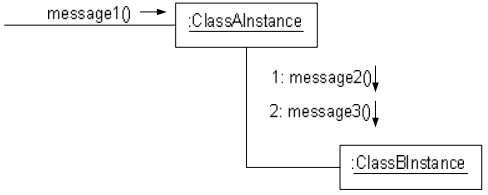
\includegraphics[width=0.5\textwidth]{foto 1.png}
\end{center}
Un diagramma di collaborazione ha il vantaggio di espandersi per vie verticali all'aggiunta di nuovi oggetti, contrariamente al chart di sequenza, il quale all'inserimento di ogni nuovo elemento tende ad espandersi orizzontalmente, per cui piuttosto limitativo.\vspace*{14pt}
\begin{center}
    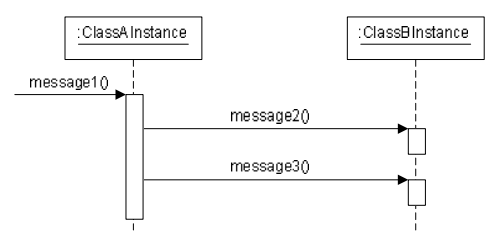
\includegraphics[width=0.5\textwidth]{foto 2.png}
\end{center}
Da canto suo, un diagramma di sequenza simile ha come aspetto positivo la facile lettura, rispetto al diagramma di collaborazione. Nonostante tale diverbio, spesso si preferisce utilizzare un diagramma che accomuni gli aspetti positivi di entrambi i charts.

\subsection*{Notazione di base}
\large
In questa sezione sono riportati tutti gli strumenti necessari per poter modellare situazioni che richiedano interazioni. Come già detto, sono indicati i costrutti principali di riferimento, caratterizzanti sia il diagramma di collaborazione ma anche di sequenza.\vspace*{14pt}\\
\textit{Definizione Lifeline}\\
Una \textbf{lifeline} è un elemento che rappresenta un partecipante individuale all'interazione. Mentre le parti e le caratteristiche strutturali possono avere moltiplicità maggiore di 1, le lifelines rappresentano soltanto una entità che interagisce.\vspace*{14pt}
\begin{center}
    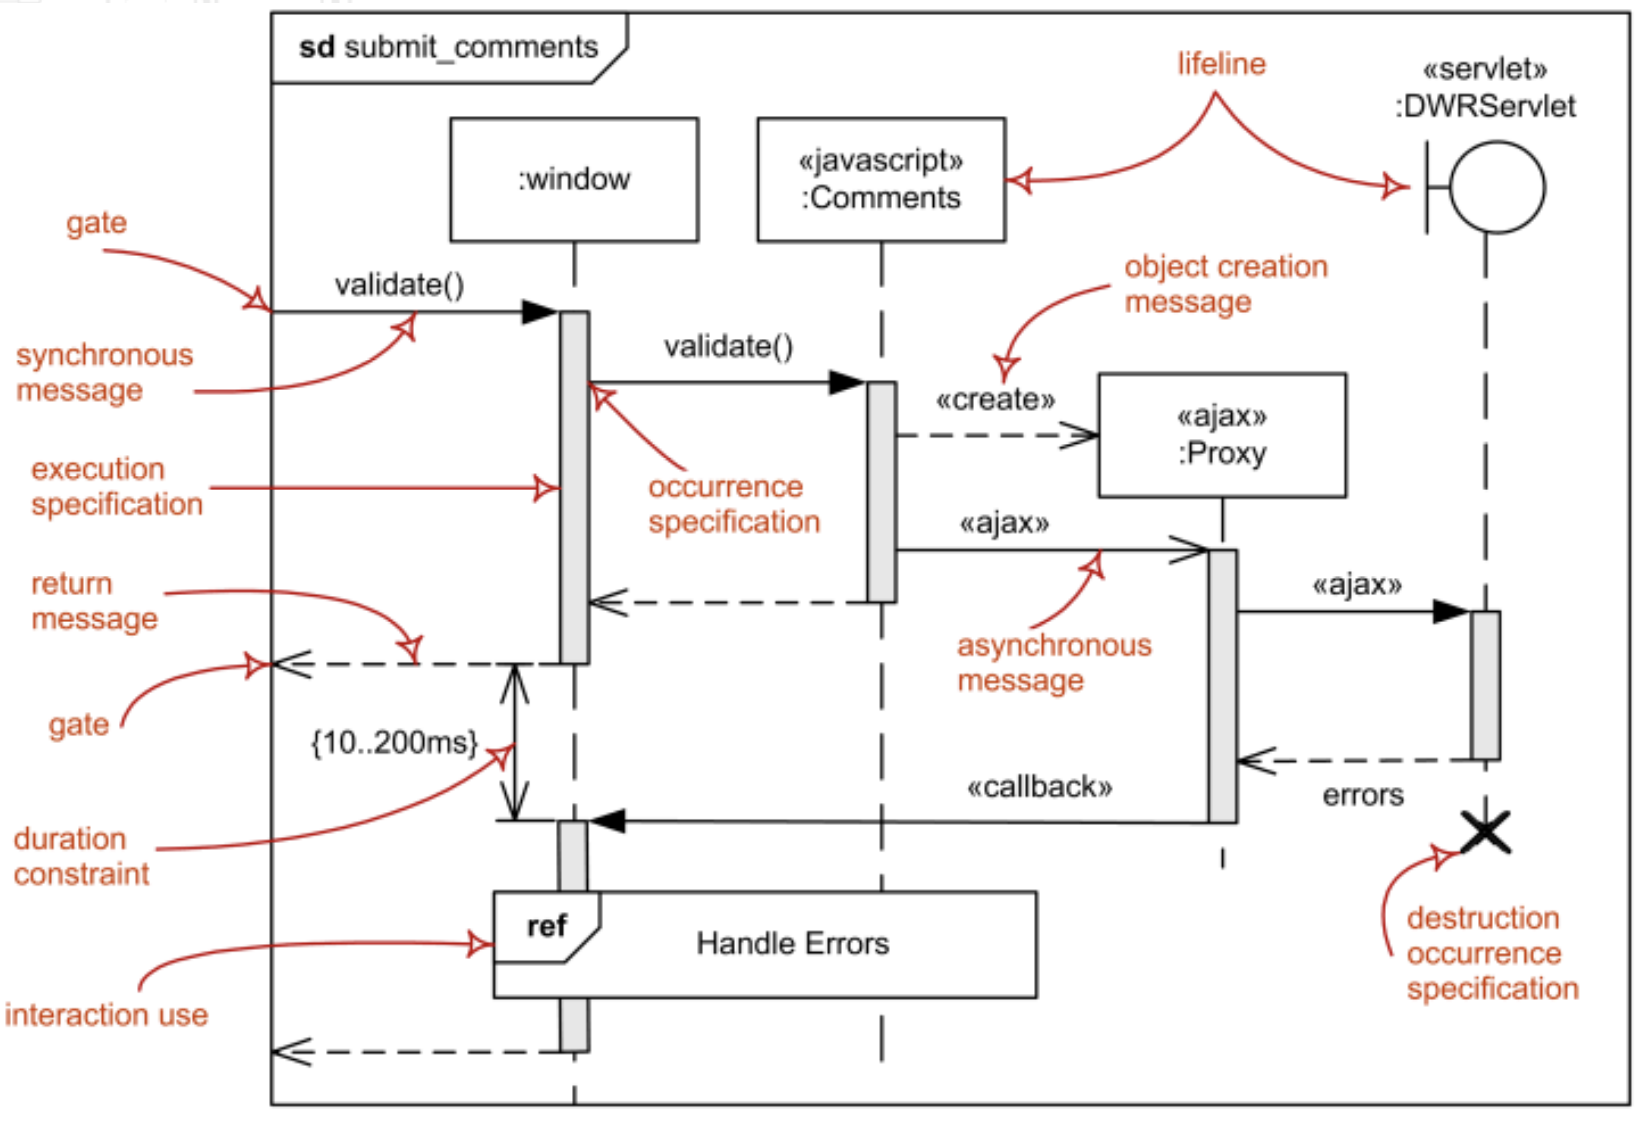
\includegraphics[width=0.4\textwidth]{foto 3.png}
\end{center}
\textit{Definizione Messaggio}\\
Un \textbf{messaggio} è una specifica comunicazione tra \textit{lifelines} che compongono una \textit{interazione}. Spesso un messaggio non riporta solamente quale sia il \textit{mittente} e il \textit{destinatario}, ma anche quale tipologia di comunicazione sia messa in atto. Tra le più disparate possibilità, un messaggio può rappresentare una chiamata ad un'operazione oppure la ricezione di un segnale. Tuttavia, in base a quale comportamento sia posto per generare il messaggio, esso viene distinto in:
\begin{enumerate}
    \renewcommand{\labelenumi}{-}
    \itemsep0em
    \item \textit{Definizione Chiamata sincrona} \begin{enumerate}[label={}]
                                \item Una \textbf{chiamata sincrona} indica una chiamata ad un'operazione. Appena inviato un messaggio è sospesa l'esecuzione dell'istanza mittente fino all'arrivo di una risposta. Tale tipologia di \textit{message} è rappresentata da una freccia direzionata con la punta ripiena.\vspace*{14pt}
                                    \begin{center}
                                        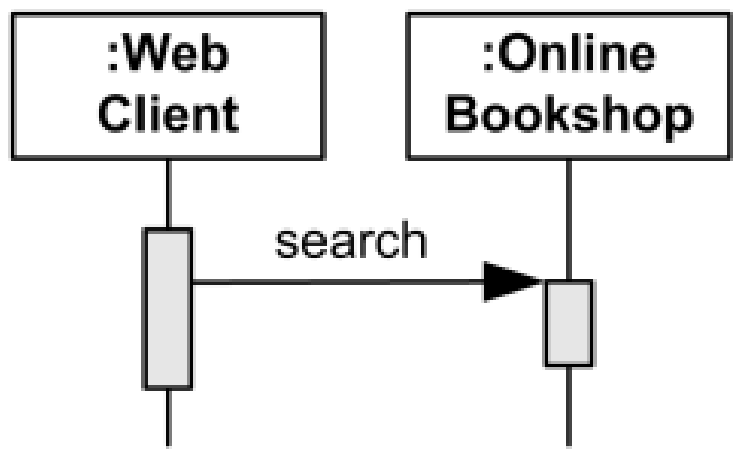
\includegraphics[width=0.2\textwidth]{foto 4.png}\\
                                    \end{center}
                            \end{enumerate}
    \item \textit{Definizione Chiamata asincrona} \begin{enumerate}[label={}]
                                \item Una \textbf{chiamata asincrona} indica anch'essa una chiamata ad un'operazione. Tuttavia, contrariamente a prima, l'invio del messaggio non implica che l'esecuzione dell'istanza sia sospesa, procede senza che attenda l'arrivo di una risposta. Questa tipologia è rappresentata mediante una freccia direzionata con la punta aperta.\vspace*{14pt}
                                    \begin{center}
                                        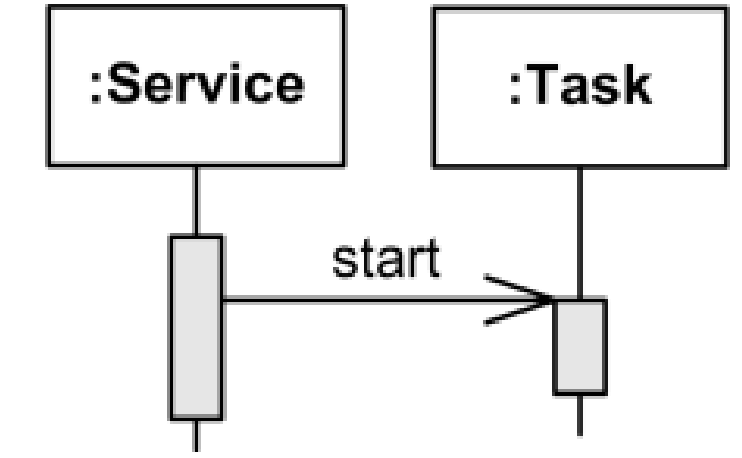
\includegraphics[width=0.2\textwidth]{foto 5.png}\\
                                    \end{center}
                            \end{enumerate}
    \item \textit{Definizione Risposta}  \begin{enumerate}[label={}]
                                \item Una \textbf{risposta} rappresenta la restituzione di dati o informazioni ad una chiamata. Rappresentata graficamente con una freccia direzionata tratteggiata, posta dal ricevitore della chiamata verso il mittente.\vspace*{14pt}
                                    \begin{center}
                                        
\includegraphics[width=0.2\textwidth]{foto 6.png}\\
                                    \end{center}
                    \end{enumerate}
    \item \textit{Definizione Creare}    \begin{enumerate}[label={}]
                                \item Indica una particolare tipologia di \textit{messaggio}, in cui una \textit{lifeline} inviando una notifica permette la creazione di una nuova \textit{istanza}.\vspace*{14pt}
                                    \begin{center}
                                        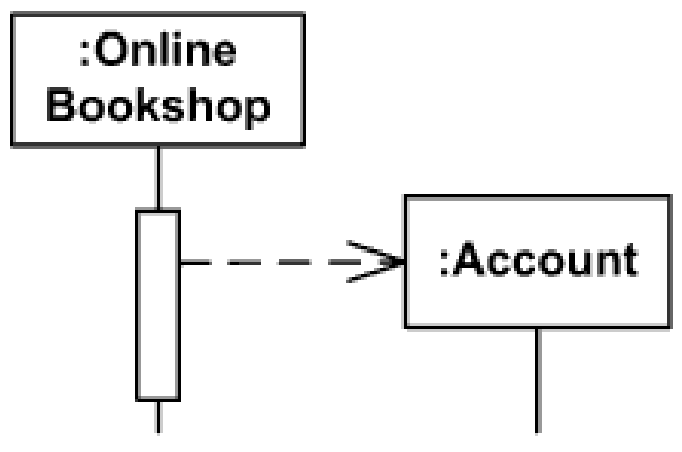
\includegraphics[width=0.2\textwidth]{foto 7.png}\\
                                    \end{center}
                    \end{enumerate}
    \item \textit{Definizione Cancellare}    \begin{enumerate}[label={}]
                                \item Un messaggio di \textbf{cancellazione} è inviato qualora si voglia terminare una determinata \textit{lifeline}. Rappresentata da una freccia direzionata ripiena, dove successivimante al termine della lifeline di riferimento è demarcata una croce che ne pone la fine.\vspace*{14pt}
                                    \begin{center}
                                        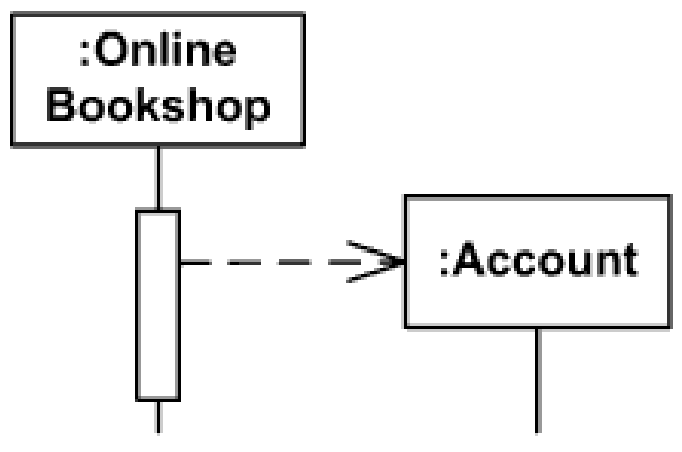
\includegraphics[width=0.2\textwidth]{foto 8.png}\\
                                    \end{center}
                        \end{enumerate}
\end{enumerate}
\textit{Definizione Lost-Found}\\
La denominazione \textbf{Lost-Found} indica un termine tecnico adoperato per una migliore e agevole lettura del diagramma di interazioni. Infatti l'obiettivo ricade nel posizionamento di certe interazioni in modo che non siano di intralcio durante la lettura degli eventi e reazioni degli oggetti dedicati; è presente, solitamente, un pallino nero iniziale che indica un successivo collegamento con un secondo pallino nero, stabilendo il proseguimento del segnale inviato o impartito.\vspace*{14pt}
\begin{center}
    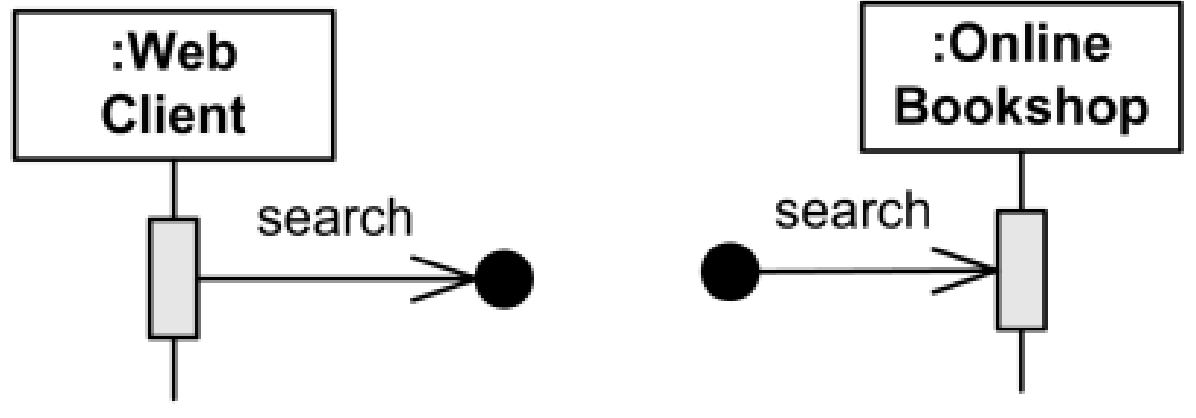
\includegraphics[width=0.4\textwidth]{foto 9.png}\\
\end{center}
\textit{Definizione Frammento di interazione}\\
Un \textbf{frammento di interazione} è un elemento che rappresenta la più generale unità di interazione. Ogni \textit{frammento di interazione} è come un'interazione a se stante. Non c'è una notazione generale per i frammenti di interazione, poichè le sue stesse sotto-classi definiscono le proprie notazioni. Alcuni esempi di frammenti di interazione sono:
\begin{enumerate}
    \renewcommand{\labelenumi}{-}
    \itemsep0em
    \item \textit{Definizione Occorenza} \begin{enumerate}[label={ }]
                        \item Un'\textbf{occorrenza} è un \textit{frammento di interazione} che rappresenta un evento preciso in cui sia descritto il ciclo di vita di un messaggio oppure di un'esecuzione.
                    \end{enumerate}
    \item \textit{Definizione Esecuzione} \begin{enumerate}[label={ }]
                        \item Un'\textbf{esecuzione} è un \textit{frammento di interazione} che rappresenta un momento precisio in cui è illustrato il \textit{lifecycle} di un'istanza, nel quale può compiere tre azioni consecutive; eseguire un'azione, conseguente ad un comportamento, mandare un segnale ad un'altra istanza oppure attendere la ricezione di una risposta, cosecutiva ad una richiesta.
                        \begin{center}
                            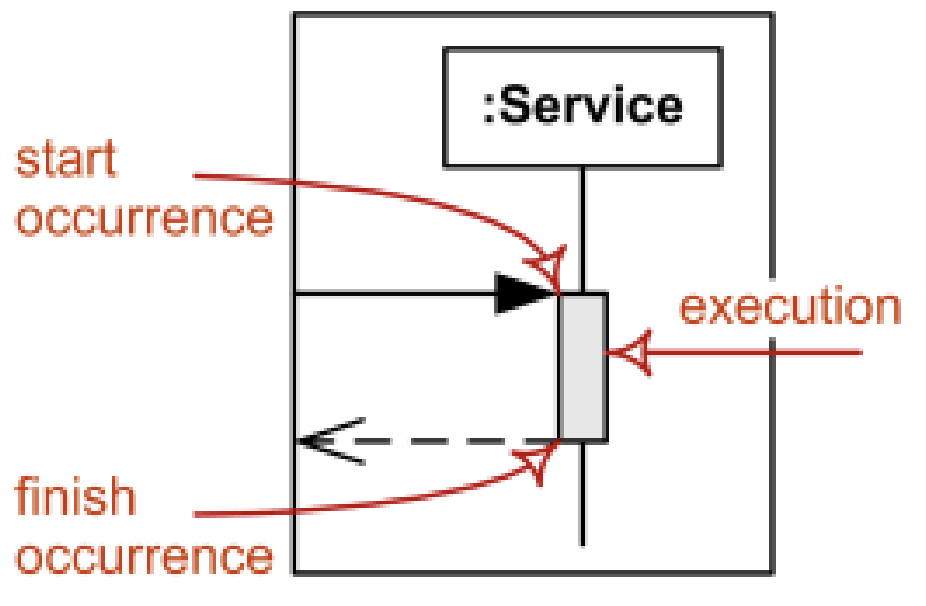
\includegraphics[width=0.4\textwidth]{foto 10.png}\\
                        \end{center}
                     \end{enumerate}
    \item \textit{Definizione Frammenti combinati} \begin{enumerate}[label={ }]
                                \item Una \textbf{combinazione di frammenti} consiste in un \textit{frammento di interazione} sommatorio, utilizzato per rendere più semplice e chiara la lettura del diagramma. 
                              \end{enumerate}
    \item \textit{Definizione Interazione d'uso} \begin{enumerate}[label={ }]
                                \item Un'\textbf{interazione d'uso} è \textit{frammento di interazione} che consente di interpellare un'ulteriore interazione. Lo scopo principale di tale sotto-classe prevede una semplificazione nell'analisi di \textit{diagrammi comportamentali}.\vspace*{14pt}
                                \begin{center}
                                    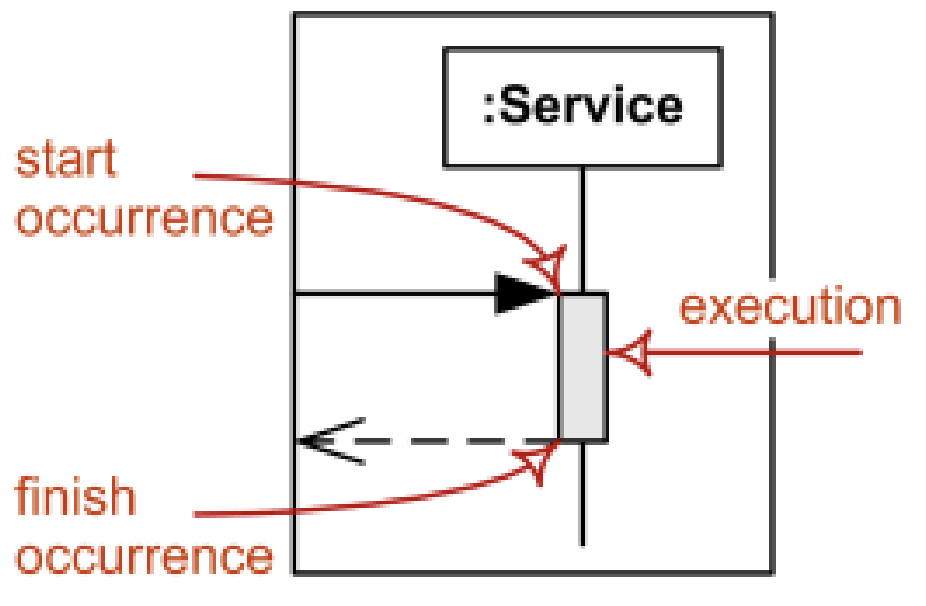
\includegraphics[width=0.3\textwidth]{foto 11.png}
                                \end{center}
                            \end{enumerate}
\end{enumerate}
\textit{Definizione Gate}\\
Un \textbf{gate} indica la \textit{fine} di un \textit{messaggio}, un punto di connessione che unisce un messaggio esterno con un messaggio interno al\textit{ frammento di interazione}.\vspace*{14pt}
\begin{center}
    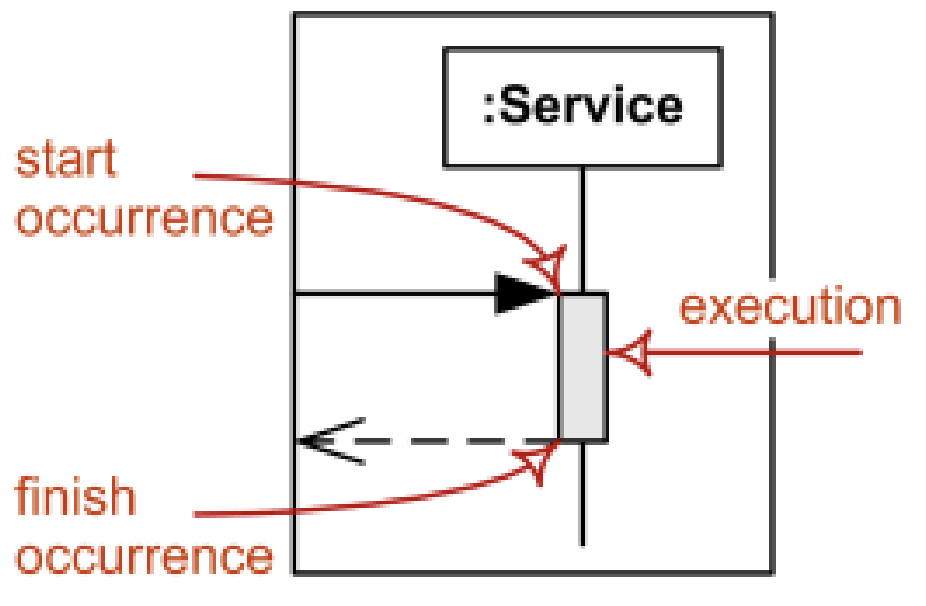
\includegraphics[width=0.3\textwidth]{foto 12.png}\\
\end{center}
\subsection*{Regole di modellazione}
\large
Un problema comune di questa tipologia di diagrammi comportamentali consiste nella quantità e specificità che gli elementi inseriti debbano possedere. Un problema relativo avviene qualora il livello di descrizione risulti essere molto vago nei confronti di istanze che richiedono un layer informativo molto più elevato.\\
Molto impegno dovrebbe essere speso per la creazione di un diagramma delle interazioni che rispecchi i dettagli trascritti all'interno dell'\textit{object design}. Tuttavia spesso questo \textit{chart} potrebbe essere imperfetto, causando una serie di modifiche durante la modellazione, ma mantiene un ruolo di fondamentale importanza, poichè è definito come un ottimo punto di partenza per indirizzare qualsiasi processo successivo di implementazione.\vspace*{14pt}\\
Regole basiche, adottate anche nei confronti di ulteriori diagrammi, sono:
\begin{enumerate}
    \renewcommand{\labelenumi}{-}
    \item Nessun messaggio tra \textit{lifelines} appartengono ad elementi del sistema
    \item Un caso d'uso può essere descritto da più di un diagramma comportamentale
    \item Il tipo di azione del messaggio può essere deciso durante la fase di \textit{design model}
\end{enumerate}
\end{document}